\chapter{Specifikacija programske potpore}
		
	\section{Funkcionalni zahtjevi}
			
			\textbf{\textit{dio 1. revizije}}\\
			
			\textit{Navesti \textbf{dionike} koji imaju \textbf{interes u ovom sustavu} ili  \textbf{su nositelji odgovornosti}. To su prije svega korisnici, ali i administratori sustava, naručitelji, razvojni tim.}\\
				
			\textit{Navesti \textbf{aktore} koji izravno \textbf{koriste} ili \textbf{komuniciraju sa sustavom}. Oni mogu imati inicijatorsku ulogu, tj. započinju određene procese u sustavu ili samo sudioničku ulogu, tj. obavljaju određeni posao. Za svakog aktora navesti funkcionalne zahtjeve koji se na njega odnose.}\\
			
			
			\noindent \textbf{Dionici:}
			
			\begin{packed_enum}
				\item Naručitelj
				\item Studenti 
				    \begin{packed_enum}
				        \item Pomagač
				        \item Traži pomoć
				    \end{packed_enum}
				\item Administrator
				\item Razvojni tim
				
			\end{packed_enum}
			
			\noindent \textbf{Aktori i njihovi funkcionalni zahtjevi:}
			
			
			\begin{packed_enum}
				\item  \underbar{Neregistrirani korisnik (inicijator) može:}
				
				\begin{packed_enum}
					
					\item pregledati listu trenutno objavljenih oglasa
					\item pregledati rejting listu studenata-pomagača
					\item filtirati oglase po smjeru, kolegiju i kategoriji
					\item se registrirati u sustav, stvoriti novi korisnicki račun za koji su mu potrebni korisničko ime, lozinka, ime, prezime, e-mail adresa i opcionalno profila slika
					
				\end{packed_enum}
			
				\item  \underbar{Registrirani korisnik (inicijator) može:}
				
				\begin{packed_enum}
					
					\item pregledati listu trenutno objavljenih oglasa
					\item pregledati rejting listu studenata-pomagača
					\item filtirati oglase po smjeru, kolegiju i kategoriji
					\item može objavljivati i odgovarati na oglase
					\item može pregledavati svoje aktivne i neaktivne oglase
					\item može uređivati ili obrisati vlastite oglase
					\item može pregledavati sve svoje trenutne upite
					\item može davati ocjenu studetnu-pomagaču
					\item može promjeniti profilnu, lozinku ili korisničko ime
					\item može izbrisati korisnički račun
					
				\end{packed_enum}
				
				\item  \underbar{Moderator (inicijator) može:}
				
				\begin{packed_enum}
					
					\item pregledati listu trenutno objavljenih oglasa
					\item pregledati rejting listu studenata-pomagača
					\item filtirati oglase po smjeru, kolegiju i kategoriji
					\item može objavljivati i odgovarati na oglase
					\item može pregledavati svoje aktivne i neaktivne oglase
					\item može uređivati ili obrisati vlastite oglase
					\item može pregledavati sve svoje trenutne upite
					\item može davati ocjenu studetnu-pomagaču
					\item može promjeniti profilnu, lozinku ili korisničko ime
					\item može izbrisati korisnički račun
					\item može brisati tuđe oglase uz dani razlog
					
				\end{packed_enum}
				
				\item  \underbar{Registrirani korisnik (inicijator) može:}
				
				\begin{packed_enum}
					
					\item pregledati listu trenutno objavljenih oglasa
					\item pregledati rejting listu studenata-pomagača
					\item filtirati oglase po smjeru, kolegiju i kategoriji
					\item može objavljivati i odgovarati na oglase
					\item može pregledavati svoje aktivne i neaktivne oglase
					\item može uređivati ili obrisati vlastite oglase
					\item može pregledavati sve svoje trenutne upite
					\item može davati ocjenu studetnu-pomagaču
					\item može promjeniti profilnu, lozinku ili korisničko ime
					\item može izbrisati korisnički račun
					
				\end{packed_enum}
				
				\item  \underbar{Baza podataka (sudionik) može:}
				
				\begin{packed_enum}
					
					\item pohranjuje sve podatke o korisnicima i njihovim ovlastima
					\item pohranjuje sve podatke o oglasima i upitima
					\item pohranjuje sve obrisane oglase (neprikladne ili obrisane od strane korisnika)
					
				\end{packed_enum}
				
				
			\end{packed_enum}
			
			\eject 
			
			
				
			\subsection{Obrasci uporabe}
				
		
					\noindent \underbar{\textbf{UC1 -Registracija}}
					\begin{packed_item}
	
						\item \textbf{Glavni sudionik: }Korisnik
						\item  \textbf{Cilj:} Stvaranje korisničkog računa 
						\item  \textbf{Sudionici:} Baza podataka
						\item  \textbf{Preduvjet:} -
						\item  \textbf{Opis osnovnog tijeka:}
						
						\item[] \begin{packed_enum}
	
							\item Neregistrirani korisnik odabire opciju za registraciju
							\item Neregistrirani korisnik unosi potrebne korisničke podatke
							\item Korisnik prima obavijest o uspješnoj registraciji
						\end{packed_enum}
						
						\item  \textbf{Opis mogućih odstupanja:}
						
						\item[] \begin{packed_item}
	
							\item[2.a] Odabir već zauzetog korisničkog imena ili neispravnog e-mail adrese, unos korisničkog podatka u nedozvoljenom formatu
							\item[] \begin{packed_enum}
								
								\item Sustav obavještava korisnika o neuspjelom upisu i vraća ga na stranicu za registraciju
								\item Korisnik mijenja potrebne podatke te završava unos ili odustaje od registracije
								
							\end{packed_enum}
						\end{packed_item}
					\end{packed_item}
					
					\noindent \underbar{\textbf{UC2 -Prijava u sustav}}
					\begin{packed_item}
	
						\item \textbf{Glavni sudionik: }Korisnik
						\item  \textbf{Cilj:} Dobiti mogućnosti interakcija s oglasima(objavljivanje, brisanje ili slanje upita)
						\item  \textbf{Sudionici:} Baza podataka
						\item  \textbf{Preduvjet:} Registracija
						\item  \textbf{Opis osnovnog tijeka:}
						
						\item[] \begin{packed_enum}
	
							\item Unos korisničkog imena i lozinke
							\item Potvrda o ispravnosti unesenih podataka
							\item Pristup korisničkim funckijama
							
						\end{packed_enum}
						
						\item  \textbf{Opis mogućih odstupanja:}
						
						\item[] \begin{packed_item}
	
							\item[2.a] Neispravno korisničko ime/lozinka
							\item[] \begin{packed_enum}
								
								\item Sustav obaviještava korisnika o neuspjelom upisu i vraća ga na stranicu za prijavu u aplikaciju

								
							\end{packed_enum}
						\end{packed_item}
					\end{packed_item}
					
					\noindent \underbar{\textbf{UC3 -Pregled oglasa}}
					\begin{packed_item}
	
						\item \textbf{Glavni sudionik: }Korisnik
						\item  \textbf{Cilj:} Pregled aktivnih oglasa
						\item  \textbf{Sudionici:} Baza podataka
						\item  \textbf{Preduvjet:} -
						\item  \textbf{Opis osnovnog tijeka:}
						
						\item[] \begin{packed_enum}
	
							\item Lista svih aktivnih oglasa je prikazana pilikom učitavanja aplikacije
							\item Mogućnost filtriranja oglasa po određenim kriterijima
							\item $<$opis korak tri$>$
							\item $<$opis korak četiri$>$
							\item $<$opis korak pet$>$
						\end{packed_enum}

					\end{packed_item}
					
					\noindent \underbar{\textbf{UC4 -Pretraga oglasa}}
					\begin{packed_item}
	
						\item \textbf{Glavni sudionik: }Korisnik
						\item  \textbf{Cilj:} Filtrirati oglase po vlastitim kriterijima
						\item  \textbf{Sudionici:} Baza podataka
						\item  \textbf{Preduvjet:} -
						\item  \textbf{Opis osnovnog tijeka:}
						
						\item[] \begin{packed_enum}
	
							\item Korisnik filtrira oglase po kriteriju kolegija, smjera i kategorije
							\item Izlistaju se oglasi koji zadovoljavaju tražene kriterije
						\end{packed_enum}
						
						\item  \textbf{Opis mogućih odstupanja:}
						
						\item[] \begin{packed_item}
	
							\item[2.a] Niti jedan oglas ne zadovoljava tražene kriterije
							\item[] \begin{packed_enum}
								
								\item Korisnika se obaviještava da nema traženog oglasa
								
							\end{packed_enum}

							
						\end{packed_item}
					\end{packed_item}
					
					\noindent \underbar{\textbf{UC5 -Uređivanje vlastitih oglasa}}
					\begin{packed_item}
	
						\item \textbf{Glavni sudionik: } Korisnik
						\item  \textbf{Cilj:} Preudrediti objavljeni oglas
						\item  \textbf{Sudionici:} Baza podataka
						\item  \textbf{Preduvjet:} 
						    \begin{packed_enum}
	
							\item Korisnik je prijavljen u sustav
							\item Oglas je aktivan
						    \end{packed_enum}
						\item  \textbf{Opis osnovnog tijeka:}
						
						\item[] \begin{packed_enum}
	
							\item Korisnik odabire opcije preuredi
							\item Preuređuje naslov/opis oglasa
							\item Odabire opciju pohrani
							\item Promjene se pohranjuju u bazu podataka
						\end{packed_enum}
						
					
					\end{packed_item}
					
					\noindent \underbar{\textbf{UC6 -Reply na oglas}}
					\begin{packed_item}
	
						\item \textbf{Glavni sudionik: } Korisnik
						\item  \textbf{Cilj:} Postaviti upit na oglas
						\item  \textbf{Sudionici:} Baza podataka
						\item  \textbf{Preduvjet:} 
						    \begin{packed_enum}
	
							\item Korisnik je prijavljen u sustav
							\item Oglas je aktivan
						    \end{packed_enum}
						\item  \textbf{Opis osnovnog tijeka:}
						
						\item[] \begin{packed_enum}
	
							\item Korisnik odabire opciju reply
							\item Korisnik unosi traženu poruku
							\item Korisniku koji je objavio oglas se šalje e-mail s upitom i kontakt podatcima zainteresiranog korisnika
							\item Upit se pohranjuje u bazu podataka
						\end{packed_enum}
						
					
					\end{packed_item}
					
					\noindent \underbar{\textbf{UC7 -Post oglas}}
					\begin{packed_item}
	
						\item \textbf{Glavni sudionik: } Korisnik
						\item  \textbf{Cilj:} Objaviti oglas
						\item  \textbf{Sudionici:} Baza podataka
						\item  \textbf{Preduvjet:} Korisnik je prijavljen u sustav

						\item  \textbf{Opis osnovnog tijeka:}
						
						\item[] \begin{packed_enum}
	
							\item Korisnik odabire opciju post 
							\item Korisnik unosi traženi naslov, opis,kolegij i kategoriju
							\item Oglas se pohranjuje u bazu podataka
						\end{packed_enum}
						
					
					\end{packed_item}
					
					\noindent \underbar{\textbf{UC8 -Ocjenjivanje studenta-pomagača}}
					\begin{packed_item}
	
						\item \textbf{Glavni sudionik: } Korisnik
						\item  \textbf{Cilj:} Ocjeniti studenta-pomagača
						\item  \textbf{Sudionici:} Baza podataka
						\item  \textbf{Preduvjet:} 
						    \begin{packed_enum}
	
							\item Korisnik je prijavljen u sustav
							\item Oglas je aktivan
							\item Oglas je tipa \textit{nudim}
							\item Reply je statusa \textit{prihvaćen}
						    \end{packed_enum}
						\item  \textbf{Opis osnovnog tijeka:}
						
						\item[] \begin{packed_enum}
	
							\item Korisnik odabire opciju ocjeni
							\item Korisnik unosi ocjenu izvrsnosti studenta-pomagača
							\item Ocjena se pribraja u dosadašnje ocjene studenta-pomagača
							\item Ocjena se pohranjuje u bazu podataka
						\end{packed_enum}
						
						\item  \textbf{Opis mogućih odstupanja:}
						
						\item[] \begin{packed_item}
	
							\item[2.a] Oglas je izbrisan
							\item[] \begin{packed_enum}
								
								\item Korisnika se obaviještava da nema mogućnost ocjene studenta-pomagača
								
							\end{packed_enum}

							
						\end{packed_item}
						
					
					\end{packed_item}
					
					\noindent \underbar{\textbf{UC9 -Pregled osobnih podataka}}
					\begin{packed_item}
	
						\item \textbf{Glavni sudionik: }Korisnik
						\item  \textbf{Cilj:} Pregledati osobne podatke
						\item  \textbf{Sudionici:} Baza podataka
						\item  \textbf{Preduvjet:} Klijent prijavljen u sustav
						\item  \textbf{Opis osnovnog tijeka:}
						
						\item[] \begin{packed_enum}
	
							\item Korisnik odabire opciju "Osobni podatci"
							\item Aplikacija prikazuje osobne podatke korisnika
						\end{packed_enum}
						
					\end{packed_item}
					
					
					
					
						\noindent \underbar{\textbf{UC10 -Promjena osobnih podataka}}
					\begin{packed_item}
	
						\item \textbf{Glavni sudionik: }Korisnik
						\item  \textbf{Cilj:} Promijeniti osobne podatke
						\item  \textbf{Sudionici:} Baza podataka
						\item  \textbf{Preduvjet:} Korisnik je prijavljen
						\item  \textbf{Opis osnovnog tijeka:}
						
						\item[] \begin{packed_enum}
	
							\item Korisnik odabere opciju za promjenu podataka
							\item Korisnik mijenja svoje osobne podatke
							\item Korisnik sprema promjene
							\item Baza podataka se ažurira

						\end{packed_enum}
						
						\item  \textbf{Opis mogućih odstupanja:}
						
						\item[] \begin{packed_item}
	
							\item[2.a] Korisnik promijeni svoje osobne podatke, ali ne odabere opciju "Spremi promjenu"
							\item[] \begin{packed_enum}
								
								\item Sustav obavještava korisnika da nije spremio podatke prije izlaska iz prozora
								
							\end{packed_enum}
							\item[2.b] Korisnik unosi već zauzeto korisničko ime
                            \item[] \begin{packed_enum}
								
								\item Sustav obavještava korisnika da je unio već zauzeto korisničko ime
								
							\end{packed_enum}
							
						\end{packed_item}
					\end{packed_item}
					
					\noindent \underbar{\textbf{UC11 -Brisanje korisničkog računa}}
					\begin{packed_item}
	
						\item \textbf{Glavni sudionik: }Korisnik
						\item  \textbf{Cilj:} zbrisati svoj korisnički račun
						\item  \textbf{Sudionici:} Baza podataka
						\item  \textbf{Preduvjet:} Korisnik je prijavljen
						\item  \textbf{Opis osnovnog tijeka:}
						
						\item[] \begin{packed_enum}
	
							\item  Korisnik pregledava osobne podatke
							\item Otvara se stranica s osobnim podacima korisnika
							\item Korisnik briše račun
							\item Korisnički račun se izbriše iz baze podataka
							\item Otvara se početna stranica
						\end{packed_enum}
					
					\end{packed_item}
					
					
                
                    \noindent \underbar{\textbf{UC12 -Brisanje oglasa}}
					\begin{packed_item}
	
						\item \textbf{Glavni sudionik: }Moderator
						\item  \textbf{Cilj:} Ukloniti neprikladne oglase
						\item  \textbf{Sudionici:} Baza podataka
						\item  \textbf{Preduvjet:} Korisnik ima ulogu moderatora
						\item  \textbf{Opis osnovnog tijeka:}
						
						\item[] \begin{packed_enum}
	
							\item Moderator primjećuje da je određenih aktivni oglas neprikladan
							\item Odabire opciju obriši te daje objašnjenje kreatoru oglasa
							\item Kreator oglasa je obaviješten putem e-mail adrese o uklanjaju oglasa
						\end{packed_enum}
						
						\item  \textbf{Opis mogućih odstupanja:}
						
						\item[] \begin{packed_item}
	
							\item[2.a] Oglas je već uklonjen ili obrisan od strane kreatora, ali je idalje vidljiv u aplikaciji
							\item[] \begin{packed_enum}
								
								\item Obavijest moderatoru da je dani oglas uklonjen

								
							\end{packed_enum}
						\end{packed_item}
					\end{packed_item}				
				
			\eject	
			\begin{fig}
			    \subsubsection{Dijagrami obrazaca uporabe}
			    
                    \graphicspath{ {slike/} }
  
                    \centering
                    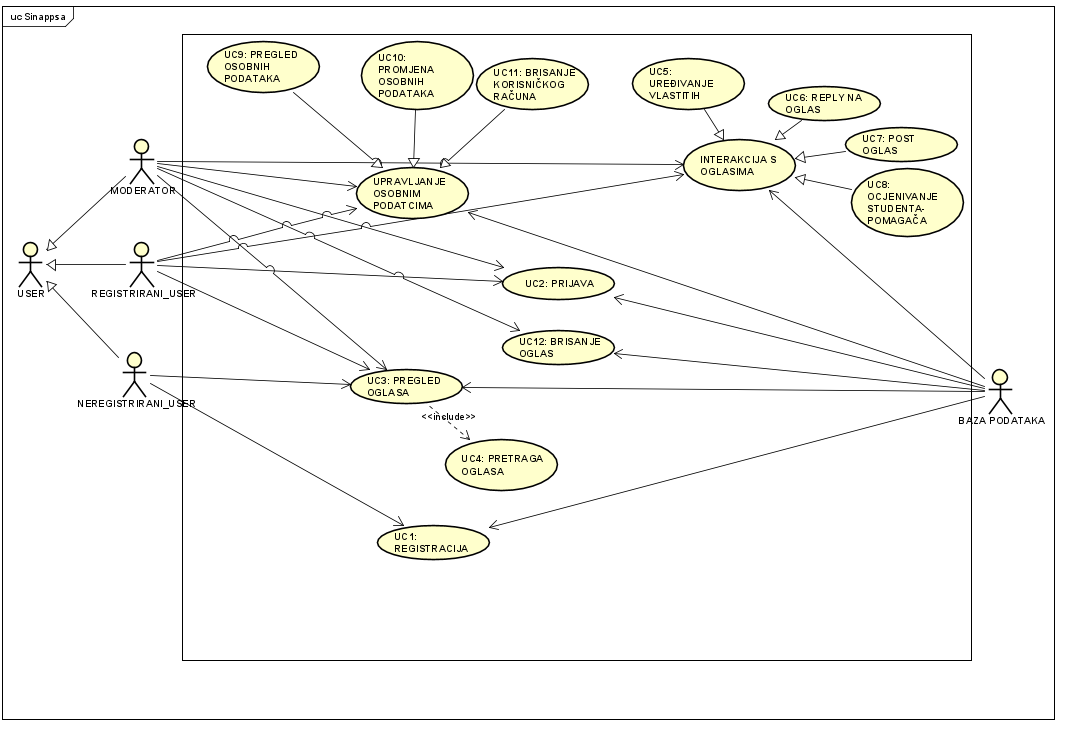
\includegraphics[width=\textwidth]{UseCase-slika.png}
                    \caption{\Slika 3.1: Dijagram obrasca uporabe registrirano korisnika, neregistriranog korisnika, moderatora i baze podataka}
               
			\eject	
			
			\end{fig}
				

			
			\subsection{Sekvencijski dijagrami}
				
				
				\noindent\textbf{Obrazac uporabe UC1-Registracija}\\
				Neregistrirani korisnik zatraži stranicu za registraciju kako bi se registirao i imao mogućnosti koje ima registrirani korisnik. Web-aplikacija mu prikazuje stranicu za registraciju. Korisnik unosi sve potrebne podatke za registraciju koje web-aplikacija zaprima i provjerava unikatnost unesenih podataka s bazom podataka točnije unikatnost e-mail adrese i username-a. Sama web-aplikacija validira valjanost podataka te korisniku vraća rezultat uspješnosti registracije. ako je registracija neuspjela vraća ga na početnu formu za registraciju. Korisnik tokom registracijskog procesa može odustati od registracije te ga web-aplikacija vraća na početnu stranicu. Nakon uspješne registracije registriranog korisnika vraća na početnu stranicu. 
				\\
                \begin{fig}
				    \graphicspath{ {slike/} }
  
                    \centering
                    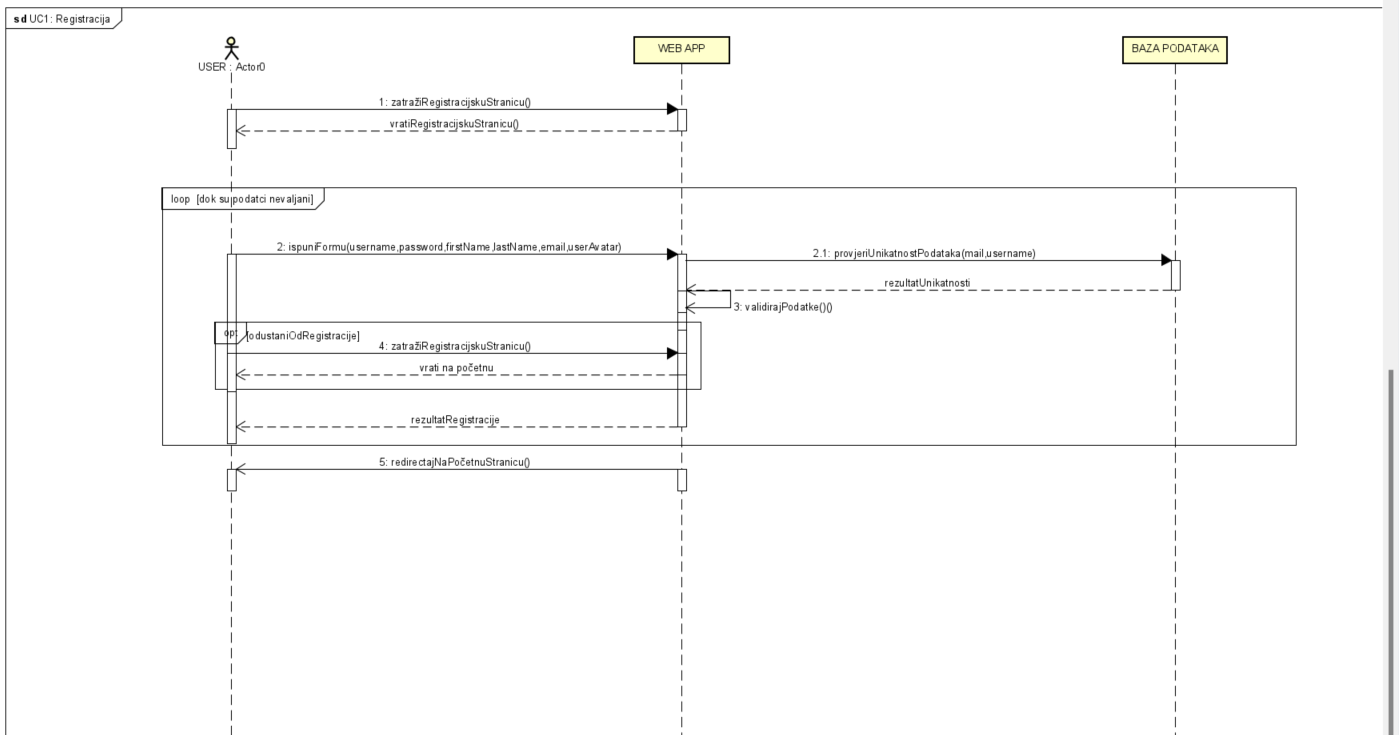
\includegraphics[width=\textwidth]{UC1_ Registracija_sekvencijskiDijagram.png}
                    \caption{\Slika 3.2: Sekvencijski dijagram za UC1}
                \end{fig}
				\\
				\\
			    \noindent\textbf{Obrazac uporabe UC6-Reply na oglas}\\
			    Korisnik koji želi postaviti upit na traženi oglas odabire opciju reply te mu web-stranica dostvlja formu za reply. Korisnik unosi proizvoljni tekst koji se predaje web-stranici, a web-stranica prosljeđuje bazi podataka kako bi baza pohranila zadani upit. Web-stranica nakon pohrane upit u bazu podatak traži od baze podatke podatke o kreatoru oglasa na koji je zadani upit postavljen kako bi kreatora oglasa putem maila obavijestila da je nekao napravio upit na njegov oglas. Web-stranica na kraju kreatoru upita daje doznanja da je mail poslan kreatoru oglasa.
			    \\
                \begin{fig}
				    \graphicspath{ {slike/} }
  
                    \centering
                    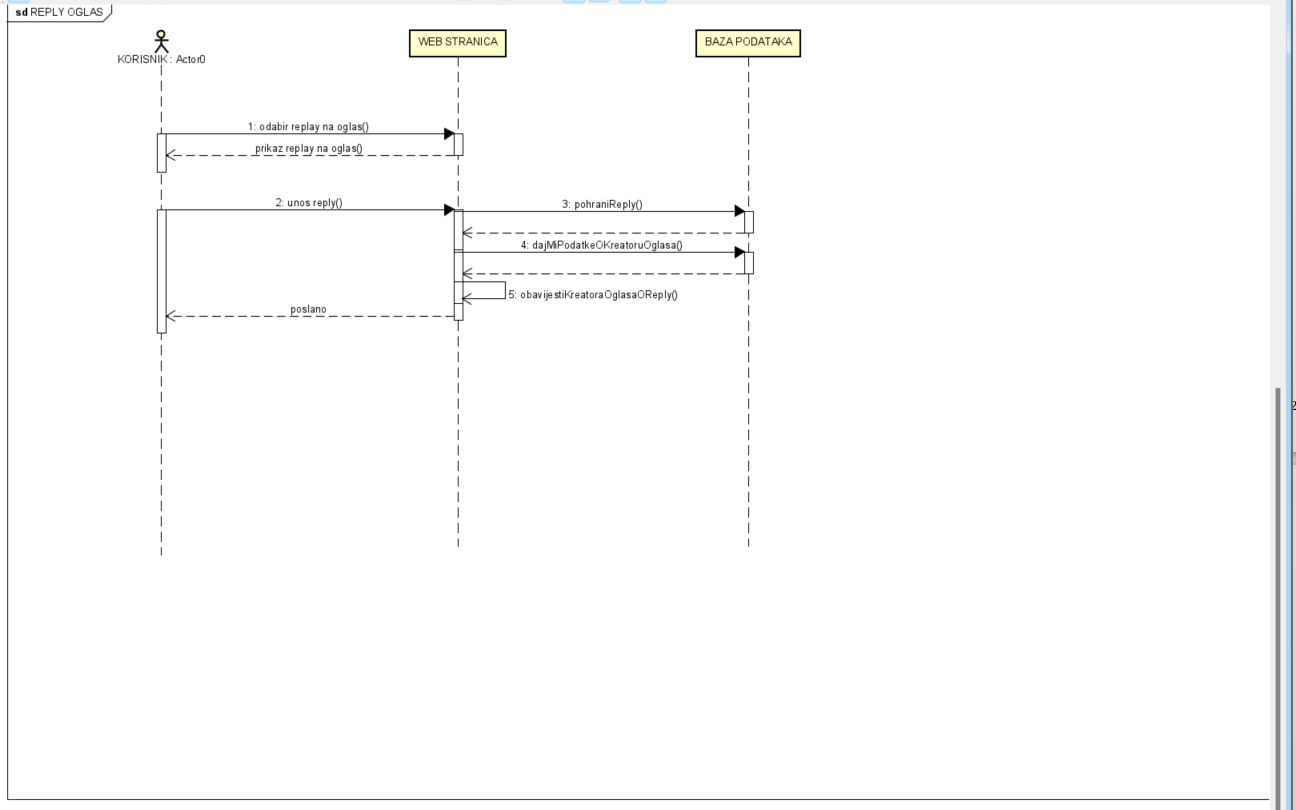
\includegraphics[width=\textwidth]{REPLY OGLAS.png}
                    \caption{\Slika 3.3: Sekvencijski dijagram za UC6}
                \end{fig}
				\\

			    \noindent\textbf{Obrazac uporabe UC7-Post oglas}\\
			    Korisnik želi objaviti oglas neovisno o samom tipu oglasa(dajem/nudim). Korisnik odabire opciju stvaranje novog oglasa te mu web-stranica vraća formu za stvaranje oglasa. Korsinik unosi podatke za oglas te unos predaje web-stranici koja provjerava valjanost unosa. Ako je unos nevaljan web-stranica vraća korisnika ponovno na formu za stvaranje oglasa ili korisnik odluči odustati od kreiranja oglasa te ga web-stranica vraća na početnu stranicu. Kada su uneseni podatci valjani korisnik objavljuje oglas te web-stranica oglas pohranjuje u bazu podataka. Na kraju web-stranica nakon uspješnog pohranjivanja oglasa u bazu podataka obaviještava korisnika da je oglas objavljen.
			    \\
			    \\
			    \begin{fig}
			   
				    \graphicspath{ {slike/} }
  
                    \centering
                    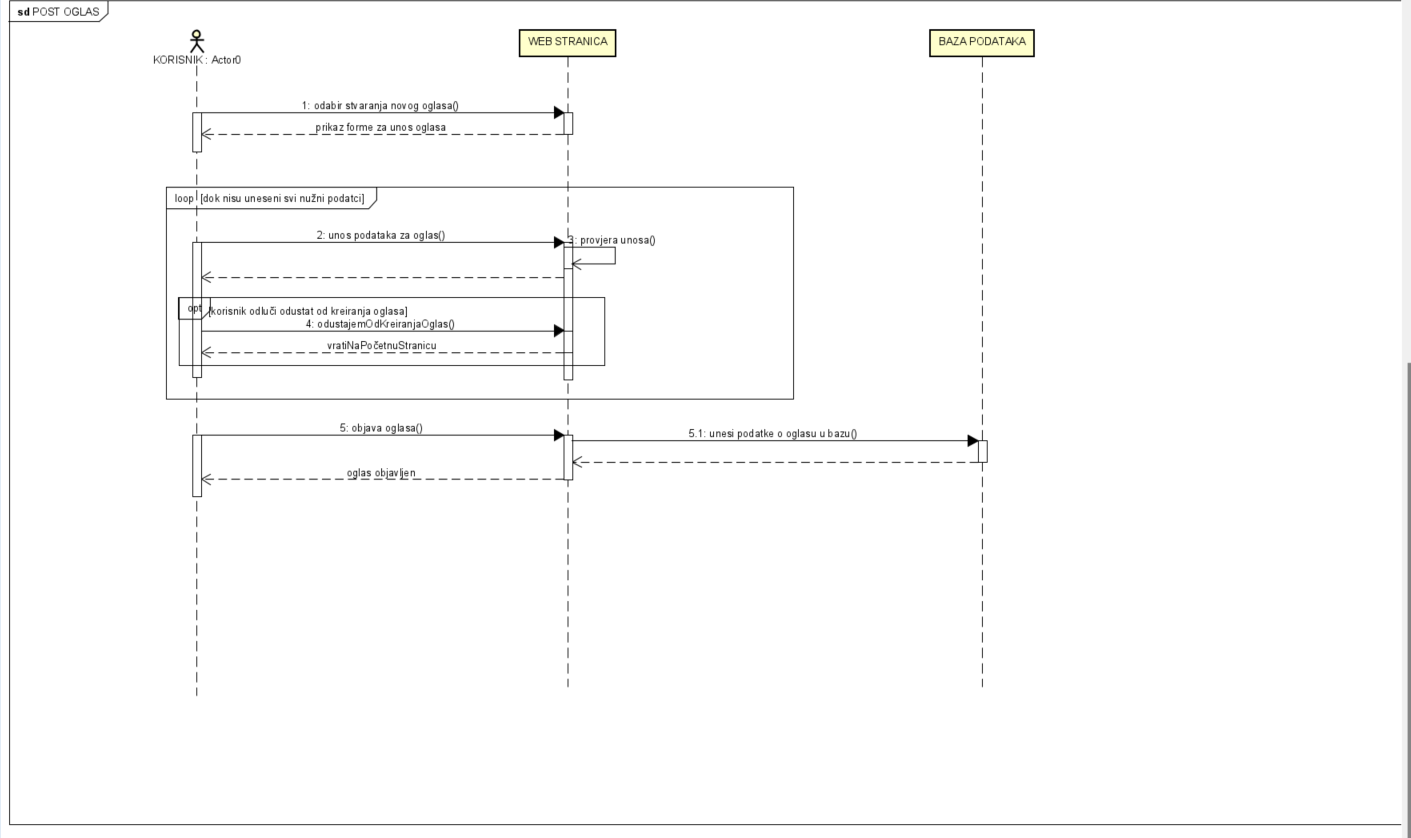
\includegraphics[width=\textwidth]{POST OGLAS.png}
                    \caption{\Slika 3.4: Sekvencijski dijagram za UC7}
                \end{fig}
			\eject

				\
	
		\section{Ostali zahtjevi}
		
			\textbf{\textit{dio 1. revizije}}\\
		 
			 \begin{packed_item}
	
			\item Sustav treba omogucitićiti rad višse korisnika u stvarnom vremenu
			\item  Korisničko sučelje i sustav moraju podržavati hrvatsku abecedu pri unosu i prikazu tekstualnog sadržaja 
			\item  Izvršavanje dijela programa u kojem se pristupa bazi podataka ne smije trajati duže od nekoliko sekundi
			\item  Sustav treba biti implementiran kao web aplikacija koristeci multiparadigmatski jezik
			\item  Sustav treba biti jednostavan za korištenje, korisnici se moraju znati koristiti sučeljem bez opširnih uputa 
			\item  Nadogradnja sustava ne smije narusavati postojeće funkcionalnosti sustava
			\item Pristup sustavu mora biti omogućen iz javne mreže pomoću HTTPS
			\item Veza s bazom podataka mora biti kvalitetno zastičena, brza i otporna na vanjske greške 
						

			\end{packed_item}
			 
			 
			 
	